\section{prinsipiell løsning}
\label{sec:concept}

Ved filterdesign kan det være lurt å ha en fornuftig arbeidsgang:

\begin{enumerate}
    \item Start med spesifikasjon
    \item Velg type filter
    \item Finn nødvendig orden $N$
    \item Finn systemfunksjonen $H(s)$
    \item Realisert $H(s)$ med tilgjengelig teknologi
  \end{enumerate}

\subsection{Spesifikasjon}
\label{sec:spesifikasjon}
Fra problembeskrivelsen i seksjon \ref{sec:issue} blir det opplyst at dersom punktprøvingsfrekvensen er $f_s$, må båndbegrensingen være $B=\frac {f_s} {2}$ og knekkfrekvensen være $f_c \geq \frac{3}{8}f_s$. Amplituderesponsen vil da ha en form tilsvarende figur \ref{fig:02ønsketamplituderespons}.

\begin{figure}[H]
	\centering
	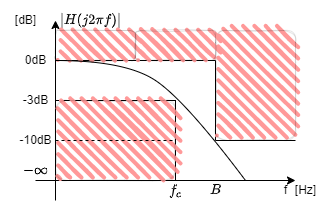
\includegraphics[scale=0.7]{./Images/02Concept/01spesifikasjon.png}
	\caption{Ønsket amplituderespons på system.\cite{pham_2022_selvlaget}}
	\label{fig:02ønsketamplituderespons}
\end{figure}

\subsection{Type filter}
\label{sec:type_filter}

For å få en amplituderespons som likner mest på figur \ref{fig:02ønsketamplituderespons} kan et Butterworth filter benyttes da den ifølge siden \cite{storr_2013_butterworth} er et analog filter som produserer den flateste amplituderesponsen, men da på bekostning av en relativt lang overgangsbånd mellom båndpass og båndstop som illustrert i figur \ref{fig:03frekvensresponsButterworth}.

\begin{figure}[H]
	\centering
	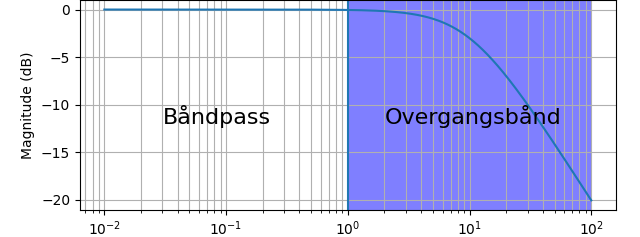
\includegraphics[scale=0.7]{./Images/02Concept/02filter.png}
	\caption{Plot av frekvensresponsen til en Butterworth lavpassfilter.\cite{pham_2022_selvlaget}}
	\label{fig:03frekvensresponsButterworth}
\end{figure}

Fra vevsiden \cite{electronicstutorials_2021_sallen} oppgis det at et 2. ordens Sallen-Key topologi som illustrert i figur \ref{fig:04SallenKey} kan brukes til å implementere forskjellige frekvens resposer som i dette tilfellet; Butterworth. Videre blir det forklart i vevsiden \cite{wikipediacontributors_2022_sallenkey} at et Butterworth filter har maksimal flat båndpass respons når Q-faktoren er lik $\frac{1}{\sqrt{2}}$, dette kan man også se på figuren \ref{fig:Qfaktor} tatt fra Electonics-Tutorials \cite{electronicstutorials_2021_sallen}. Q-faktoren er gitt ved formelen \ref{eq:Q-faktor} der $\omega_0$ er knekkfrekvensen, mens $\zeta$ er dempningsfaktoren. 

\begin{equation}
	Q=\frac{\omega_0}{2\zeta}
	\label{eq:Q-faktor}
\end{equation}


\begin{figure}[H]
	\centering
	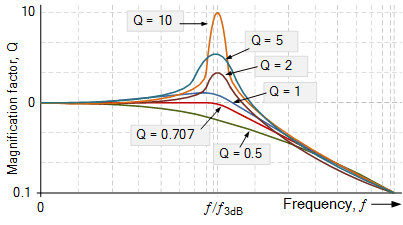
\includegraphics[scale=0.7]{./Images/02Concept/Qfaktor.png}
	\caption{Sallen key frekvens respons ved forskjellige Q-faktorer.\cite{electronicstutorials_2021_sallen}}
	\label{fig:Qfaktor}
\end{figure}


\begin{figure}[H]
	\centering
	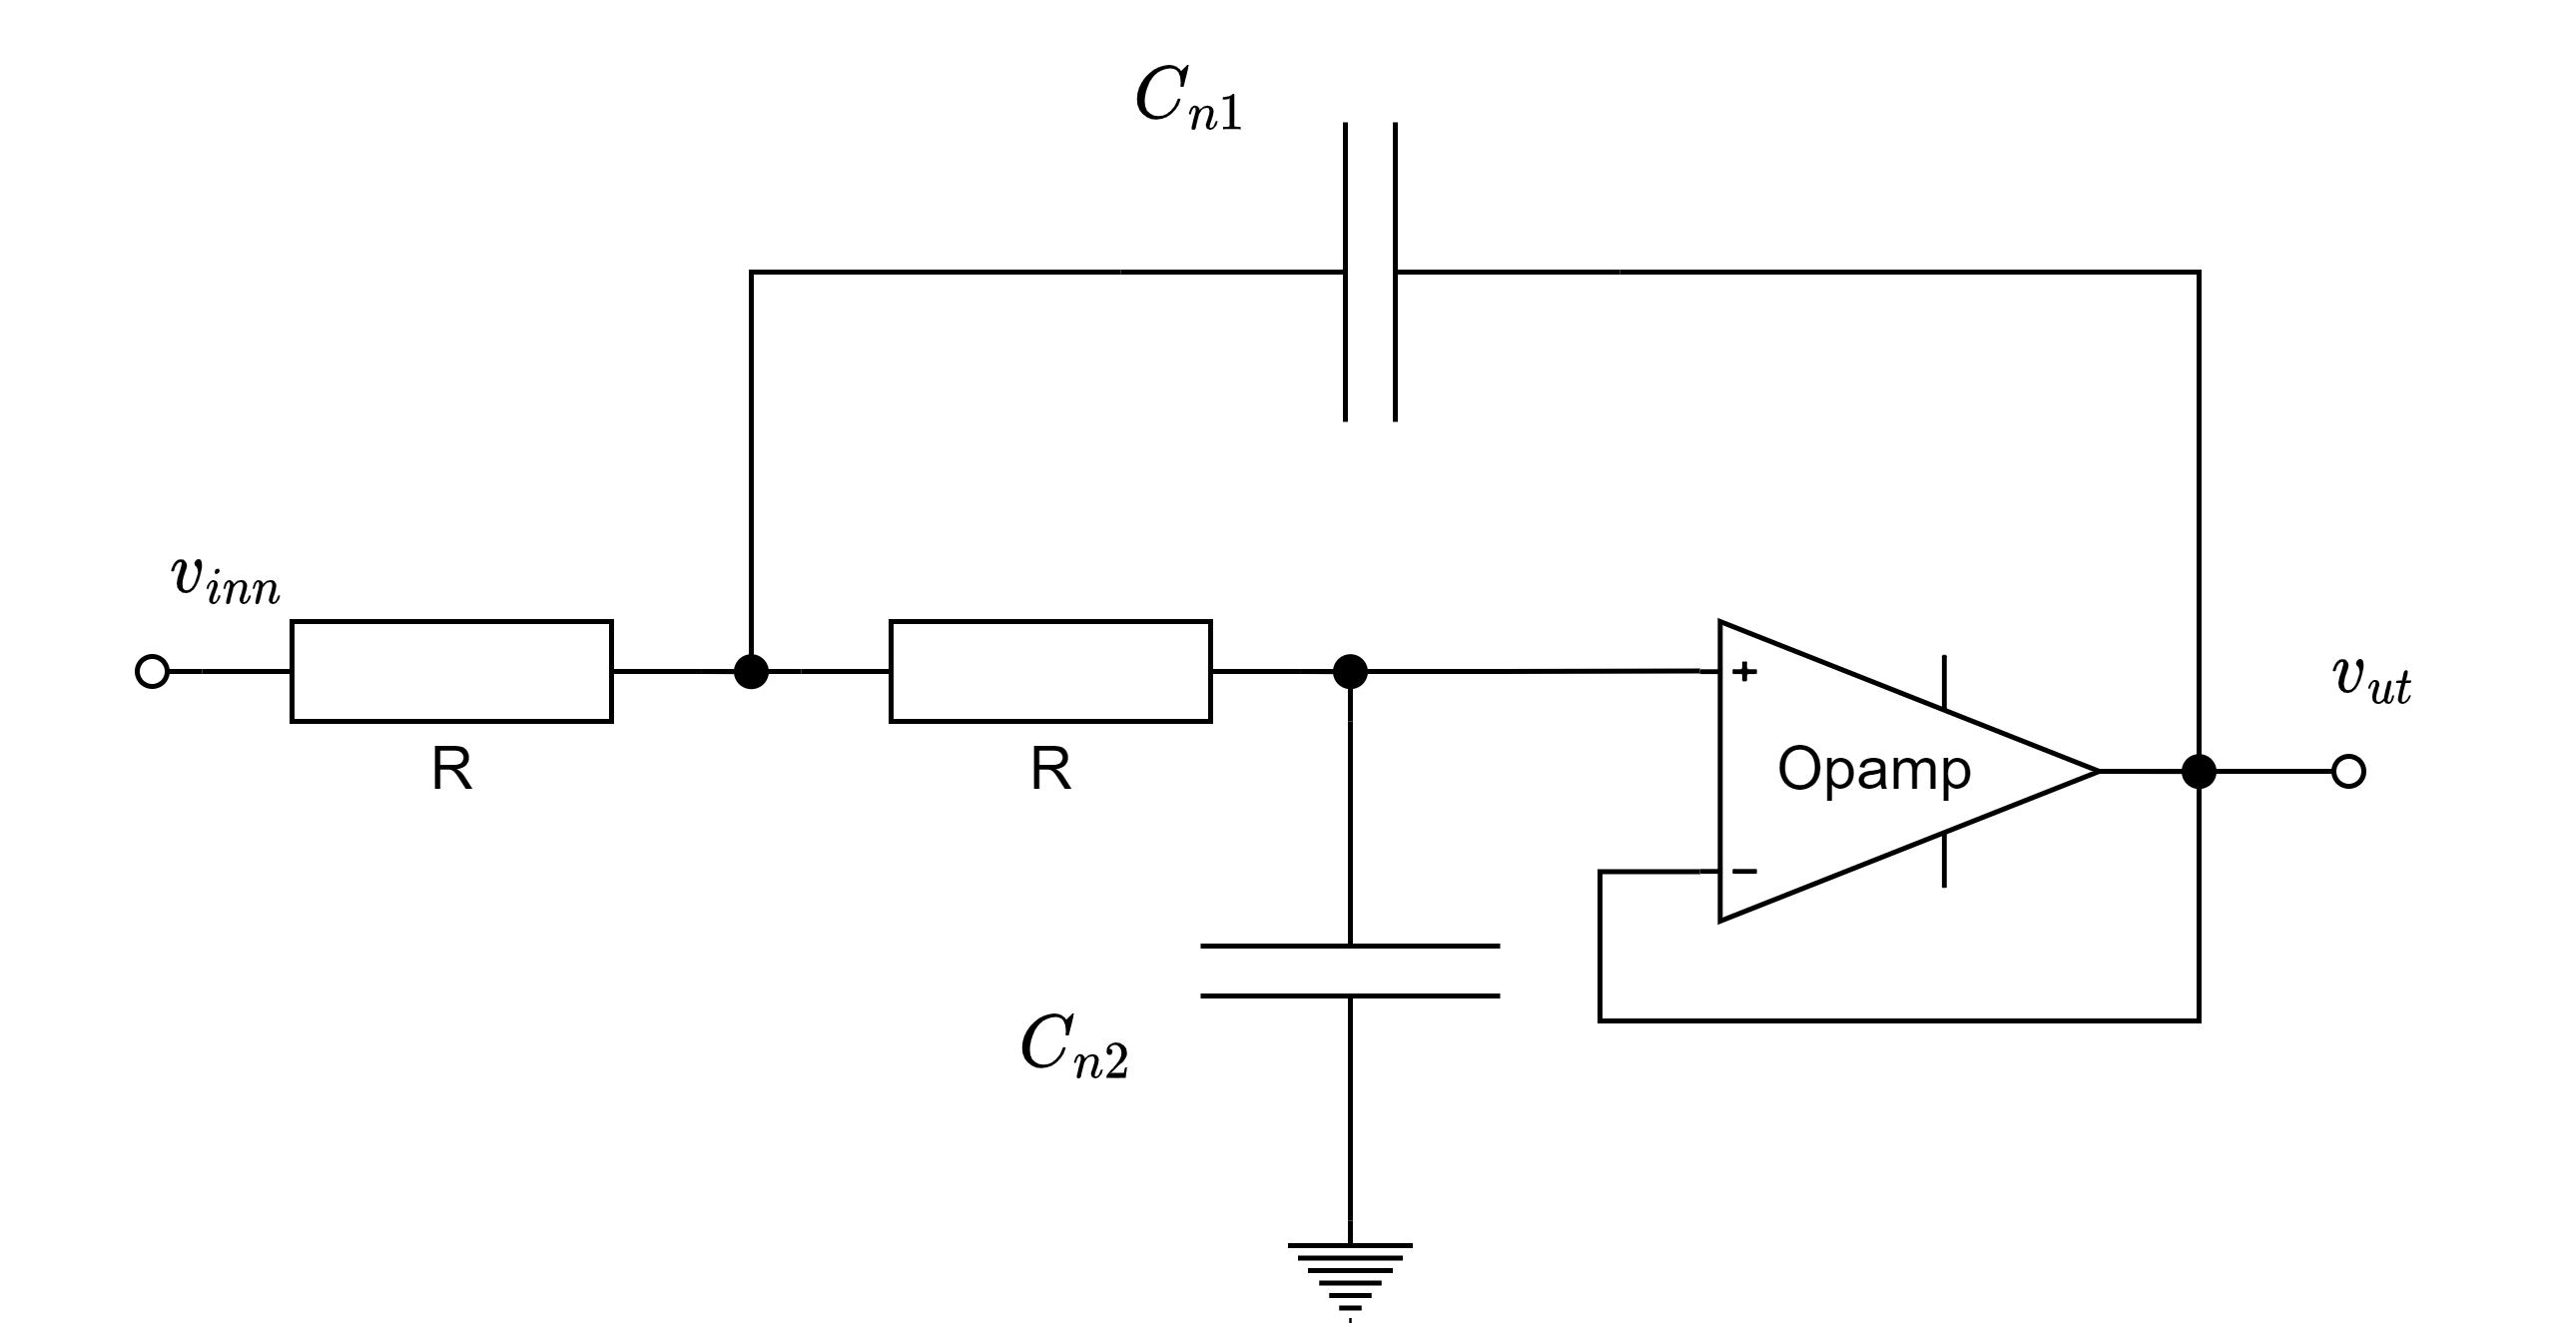
\includegraphics[scale=0.15]{./Images/02Concept/03SallenKey.png}
	\caption{Lavpassfilter med Sallen-Key topologi.\cite{pham_2022_selvlaget}}
	\label{fig:04SallenKey}
\end{figure}

\subsection{Nødvendig orden}
\label{sec:Nødvendig_orden}

Fra siden \cite{wikipediacontributors_2022_butterworth} blir det oppgitt at formelen for demping $A(\omega)$ for en $n$te-ordens Butterworth lavpassfilter er gitt ved systemfunksjonen $H(s)$ som

\begin{equation}
	A(\omega)=|H(j2\pi f)|=\frac{1}{\sqrt{1+(\frac{f}{f_c})^{2n}}}
	\label{eq:magnitude}
\end{equation}


Formel \ref{eq:magnitude} kan videre skrives om til

\begin{equation}
	n=\frac{1}{2}\frac{\ln(A^{-2}-1)}{\ln(\frac{f}{f_c})}
	\label{eq:order}
\end{equation}

Der dempingen $A$ er amplitudeforholdet, dette får man ved å bruke formelen

\begin{equation}
	A=10^{\frac{A[dB]}{20}}
	\label{eq:decibeltonone}
\end{equation}

Som man kan se på figur \ref{fig:05order} tatt fra Wikipedia \cite{wikipediacontributors_2022_butterworth} kan man se at man får et mye brattere jo høyere orden det er i filteret, men ettervert som man kommer i en høyere orden så vil også graden den blir brattere minkes. 

\begin{figure}[H]
	\centering
	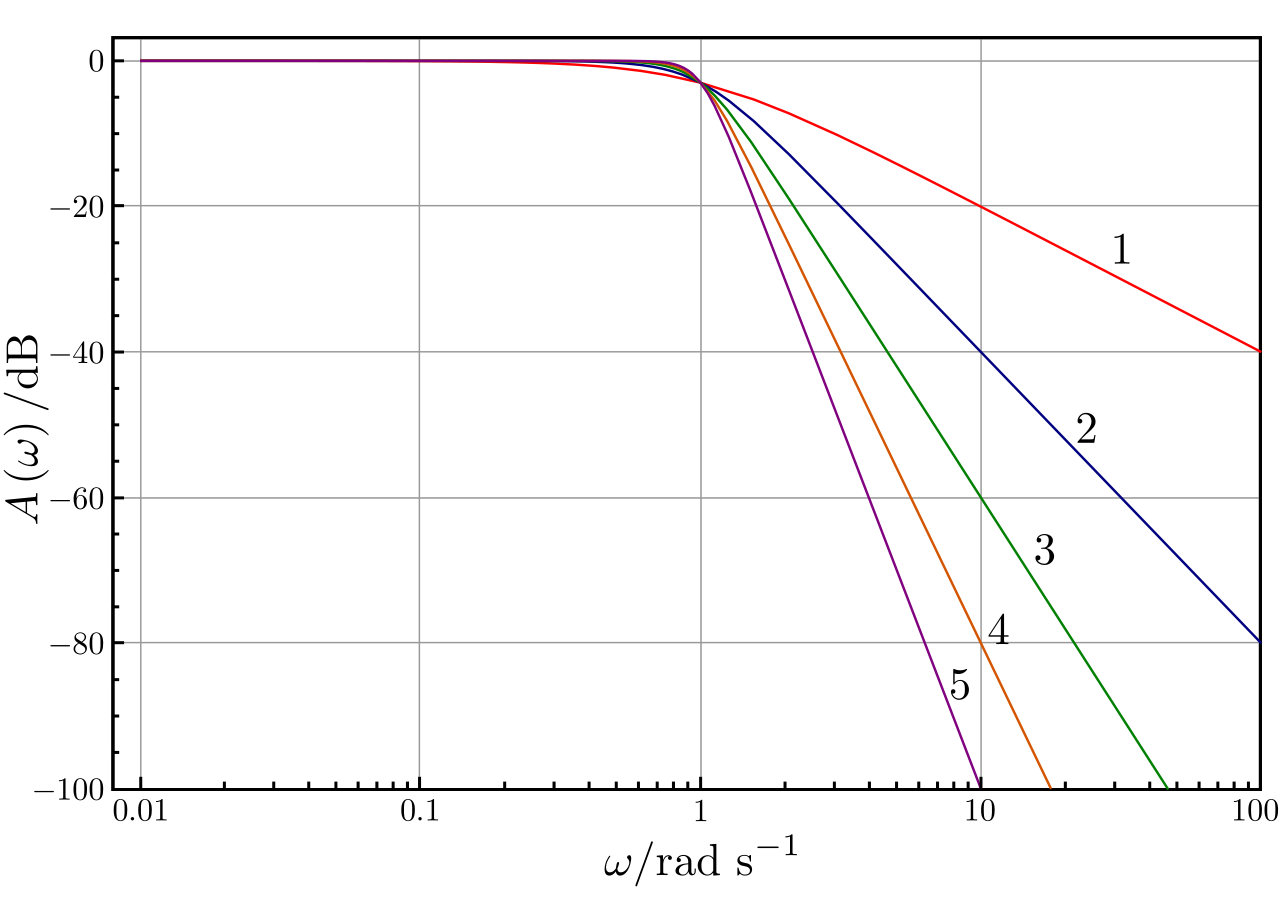
\includegraphics[scale=0.2]{./Images/02Concept/04orders.png}
	\caption{Plot med demping for et Butterworth lavpassfilter fra 1. til 5. orden med knekkfrekvens $\omega=1$.\cite{wikipediacontributors_2022_butterworth}}
	\label{fig:05order}
\end{figure}

\newpage

\subsection{Systemfunksjonen}
\label{sec:Systemfunksjonen}

Når man ved hjelp av formelen \ref{eq:order} har kommet fram til $n$-antall orden kan man ta i bruk formel \ref{eq:dempningsfaktor} oppgitt i videoen \cite{lundheim_butterworth} for å finne den relative dempningsfaktoren $\zeta$. Her er $i$ gitt for polpar. På figur \ref{fig:polezeroplot} kan man også se at polene ligger jevnt fordelt på halvsirkelen med en radius lik $\omega_0$ der vinkelen mellom polene er $\theta=\frac{\pi}{n}$. Dette gir et filter som er maskimalt flatt ifølge videoen \cite{lundheim}.

\begin{figure}[H]
	\centering
	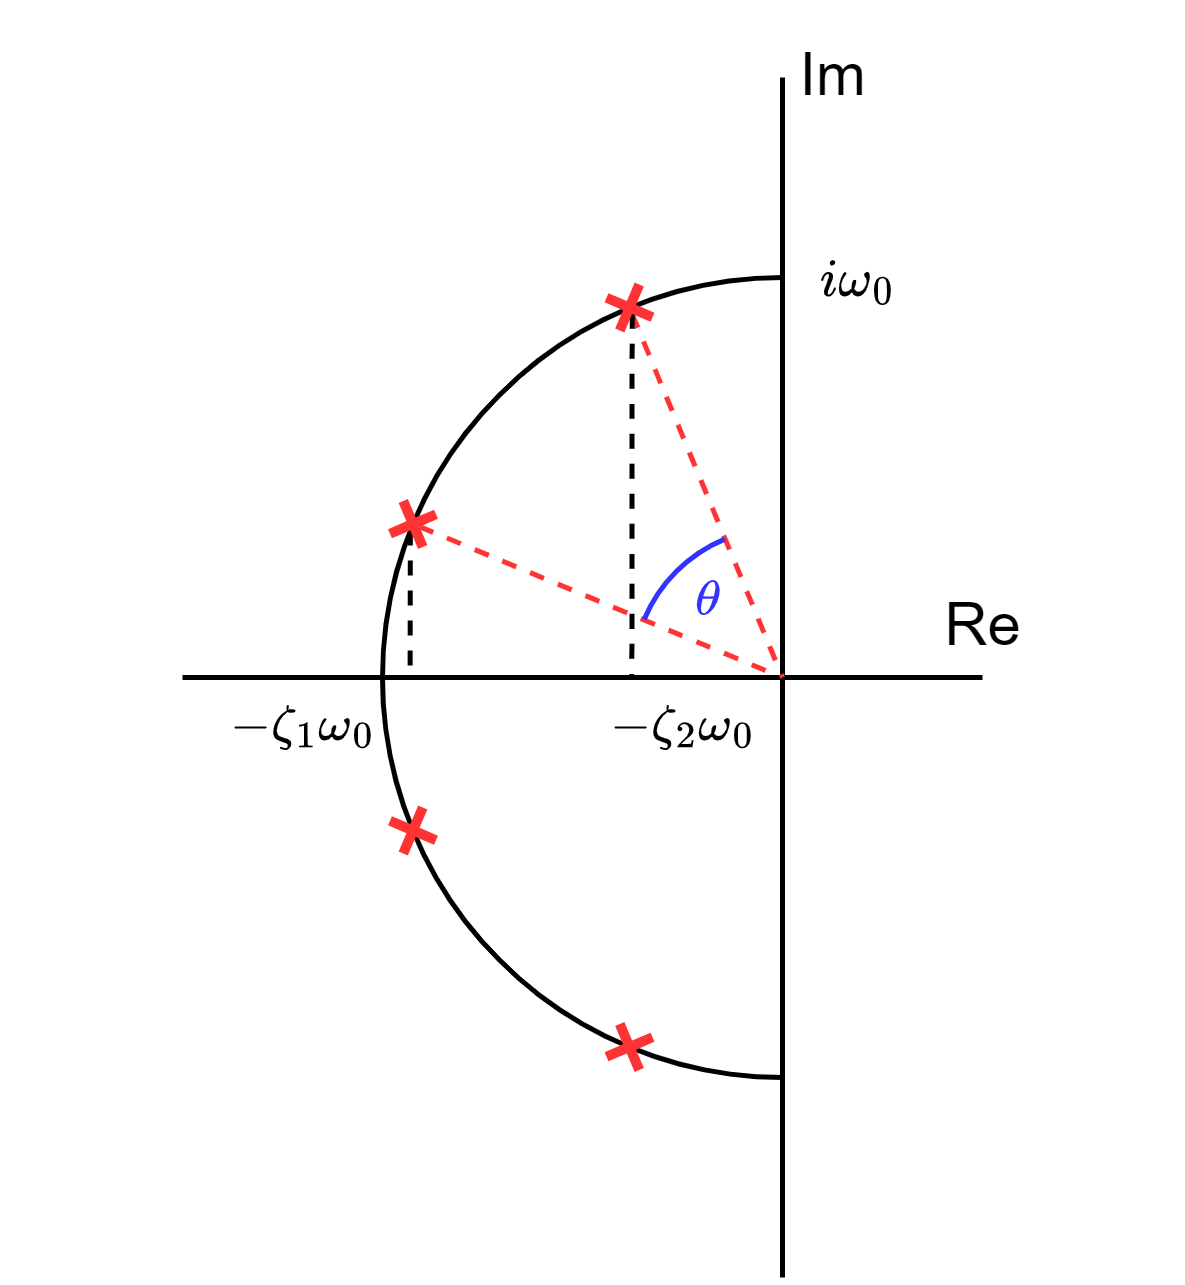
\includegraphics[scale=0.2]{./Images/02Concept/polplott.png}
	\caption{Polplott for et 4. ordens filter.\cite{pham_2022_selvlaget}}
	\label{fig:polezeroplot}
\end{figure}

\begin{equation}
	\zeta_i= \biggl\{ {{\cos\frac{\pi}{n}i \;\;\;\;\;\;\;\;\;\;\;\;\;\;\;\;\; \text{ for } n \text{ odde}} \atop {\cos [\frac{\pi}{2n}+(i-1)\frac{\pi}{n}] \: \text{ for } n \text{ like}}}
	\label{eq:dempningsfaktor}
\end{equation}

Fra videoene \cite{lundheim_2022_et} \cite{larslundheim_2022_peter2} blir det oppgitt at at tidskontstantene $\tau_{nm}=C_{nm} \cdot R$ må oppfylle kravene:

\noindent\begin{minipage}{.5\linewidth}
	\begin{equation}
		\tau_{n1}=\frac{1}{\omega_0 \zeta_n} 
	\end{equation}
	\end{minipage}%
	\begin{minipage}{.5\linewidth}
	\begin{equation}
		\tau_{n2}=\frac{1}{\omega_0^2 \tau_{n1}}
	\end{equation}
	\label{eq:tau}
	\end{minipage}

Kondensatorverdiene blir da gitt ved

\noindent\begin{minipage}{.5\linewidth}
	\begin{equation}
		C_{n1}= \frac{\tau_{n1}}{R} 
	\end{equation}
	\end{minipage}%
	\begin{minipage}{.5\linewidth}
	\begin{equation}
		C_{n2}= \frac{\tau_{n2}}{R} 
	\end{equation}
	\label{eq:capacitor}
	\end{minipage}